\section{Experimental validation}
\label{sec:validation}

In the previous section, we provided an end-to-end explanation of how the model produces a high logit difference between IO and S on the IOI task. Yet Section \ref{sec:distributed_name_movers} shows that our experimental methods do not fully account for all name-moving in the model: some new heads take on this role after the main Name Mover Heads are knocked out. We therefore seek more systematic validations to check that our account in Section~\ref{sec:circuits} includes all components used by the model to perform IOI.
%In order to validate that we did not miss anything in our circuit, our high level goals were to check if our circuit is responsible for the performance on the IOI task and if it includes all the components used by the model to perform IOI.

To formalize this, we first introduce notation to measure the performance of a circuit $C$ on the IOI task. % introduce criteria that depend on a measure $F$ of the performance of a circuit on a task. 
Suppose $X\sim \pioi$, and $f(C(X); X)$ is the logit difference between the IO and S tokens when the circuit $C$ is run on the input $X$ (recall that $C(X)$ is defined by knocking out all nodes outside $C$, as described in Section~\ref{sec:knockouts}). We define the average logit difference $F(C) \eqdef \mathbb{E}_{X \sim \pioi} \left[f(C(X); X) \right]$ as a measure of how well $C$ performs the IOI task.

%\begin{definition}
% The \emph{circuit distance metric} $\Delta$ is defined by
% \begin{equation}
% \Delta(C_1, C_2) \eqdef \mathbb{E}_{X \sim \pioi} \left[ \left| f(C_1(X); X) - f(C_2(X); X) \right| \right].
% \label{eqn:delta_distance}
% \end{equation}
%\label{def:delta}
%\end{definition}
%
% Thus, $\Delta$ checks whether two circuits consistently have similar logit difference across different samples from $\pioi$. 
Using $F$, we introduce three criteria for validating a circuit $C$. The first one, \textbf{faithfulness}, asks that $C$ has similar performance to the full model $M$, as measured by $|F(M) - F(C)|$. For the circuit $C$ from Figure~\ref{fig:the_circuit}, we find that $|F(M)-F(C)| = 0.46$, or only $13\%$ of $F(M)=3.56$. In other words, $C$ achieves $87\%$ of the performance of $M$.

However, as the Backup Name Mover Heads illustrate, faithfulness alone is not enough to ensure a complete account. In Section~\ref{sec:completeness} we introduce a toy example that illustrates this issue in more detail and use this to define two other criteria---completeness and minimality---for checking our circuit.
%of a model $M$ for which faithfulness is not sufficient to prescribe which circuits $C \subseteq M$ explain model behavior well. This motivates the criteria of completeness and minimality that we then check on our circuit.

% The equation for $x$ is $2$. For $x*$, $n$ can be calculated for $\rho$ and we can now calculate $v^2\cdot \dots$ for those that represent the constants

%Since $f(C(X); X)$ should be similar for circuits that implement the same behavior, an initial check that a circuit $C$ is implementing the same behavior as $M$ is whether $\Delta(M, C)$ is small - in which case, we call the circuit faithful. Our circuit $C$ has $\Delta(C,M) = 0.2$, and since the logit difference for the model is 3.39 our circuit is indeed faithful. 



\subsection{Completeness}
\label{sec:completeness}

% To resolve the issue that $C$ may compute an algorithm in $M$ using a different set of nodes to $M$, we need introduce a new criterion. Knocking out the same set of nodes $K$ from $C$ and $M$ should lead to the same effect on model performance, measured by $F$.

As a running example, suppose a model $M$ uses two identical and disjoint serial circuits $C_1$ and $C_2$. The two sub-circuits are run in parallel before applying an OR operation to their results. Identifying only one of the circuits is enough to achieve faithfulness, but we want explanations that include both $C_1$ and $C_2$, since these are both used in the model's computation.

% To resolve the issue that $C$ may compute an algorithm in $M$ using a different set of nodes to $M$, we need introduce a new criterion. Knocking out the same set of nodes $K$ from $C$ and $M$ should lead to the same effect on model performance, measured by $F$.

To solve this problem, we introduce the \textbf{completeness} criterion: for every subset $K \subseteq C$, the \emph{incompleteness score} $|F(C \setminus K) - F(M\setminus K)|$ should be small. In other words, $C$ and $M$ should not just be similar, but remain similar under knockouts. 

% \begin{definition}
% For a circuit $C$ and a subset $K \subseteq C$, define the \textbf{completeness score} as $\Delta(C\setminus K, M\setminus K)$. We call a circuit \textbf{$\varepsilon$-complete} if $\forall K \subseteq C, \Delta(C\setminus K, M\setminus K) \le \varepsilon$.
% \label{def:completeness}
% \end{definition}
In our running example, we can show that  $C_1$ is not complete by setting $K=C_1$. Then $C_1 \setminus K$ is the empty circuit while $M\setminus K$ still contains $C_2$. The metric $|F(C_1 \setminus K)- F(M \setminus K)|$ will be large because $C_1 \setminus K$ has trivial performance while $M \setminus K$ successfully performs the task.
%In this case the completeness score will be large, and thus the partial explanation will not pass the completeness test. 
%However, this definition doesn't cover all cases of ``incompleteness'' we would wish to cover\footnote{If two nodes in $M \setminus K$ perfectly cancel each other, independent from $C$ then the completeness definition could be met without including either of these important nodes in a circuit. We could also check that $F(C)$ doesn't change after adding nodes: $\forall K \subseteq M, |F(C \cup K) - F(M)| \leq \varepsilon.$ However, in practice such cases of compensation are improbable.}.

% NEW COMPLETENESS
% In this section, we clarify how to empirically check our criterion of completeness and present the results of this justification. To satisfy completeness (equation (\ref{eqn:completeness})), we need to evaluate an expectation over $K \subseteq C$, and since $2^{|C|}$ the number of subsets of $C$ is too large to iterate over, we estimate the expectation with random saampling. Additionally, to ensure there aren't subsets that have high completeness score but are not found with random sampling, we also check $K$ equal to the all nodes in each of the circuit classes.
% END NEW COMPLETENESS

Testing completeness requires a search over exponentially many subsets $K \subseteq C$. This is computationally intractable given the size of our circuit, hence we use three sampling methods to seek sets $K$ that give large incompleteness scores:
\begin{compactitem}
\item The first sampling method chooses subsets $K \subseteq C$ uniformly at random.
\item The second sampling method set $K$ to be an entire class of circuit heads $G$, e.g the Name Mover Heads. $C \setminus G$ should have low performance since it's missing a key component, whereas $M \setminus G$ might still do well if it has redundant components that fill in for $G$. %In this case, $\Delta(C \setminus G, C)$ is likely to be large, since the circuit is missing a crucial component.  while $\Delta(M \setminus G, C)$ may be small if $M \setminus G$ contains even one node that can perform the same function as the class $G$ (i.e we ``missed'' this node in our circuit). Together, these would imply that $\Delta(C\setminus G,M\setminus G)$ is large and may be close to the circuit's completeness score.
\item Thirdly, we greedily optimized $K$ node-by-node to maximize the incompleteness score (see Appendix \ref{app:greedy} for details).
\end{compactitem}
All results are shown in Figure \ref{fig:completenessA}.
The first two methods of sampling $K$ suggested to us that our circuit was complete, as every incompleteness score computed with those methods was small.  However, the third resulted in sets $K$ that had high incompleteness score: up to 3.09 (87\% of the original logit difference). These greedily-found sets were usually not semantically interpretable (containing heads from multiple categories), and investigating them would be an interesting direction of future work.
% and 3.03 for the naive circuit (this represents 85\% of $F(M)$). The full details of the greedy approach and the interpretation of the $K$ found can be found in Appendix \ref{app:greedy}. We hope further work can find out the limitation of our metric choice, or explanations robust to this adversarial completeness check.

%The results in Figure \ref{fig:completeness} suggest that our circuit could be $\varepsilon$-complete for $\varepsilon = $\todo{}, which is a noticeable improvement over the naive circuit which is only $\varepsilon$-complete for $\varepsilon \ge$\todo{}.

% For each set $K$, we computed an empirical completeness score, $\mathbb{E}_{X \sim \pioi}[|\mathrm{LD}_{C\setminus K}(X) -  \mathrm{LD}_{M\setminus K}(X)|]$ where $\mathrm{LD}_{C}$ \ac{not a fan of this notation, think its overwhelming} denote the logit difference of the output of $C$ on the sample $X$. As shown in figure (\ref{fig:completeness}), all the sets found by both methods have score less than $1.4$ (39\% of the original logit difference). This gives a lower bound on the actual $\varepsilon$ that characterize the circuit completeness. \todo{add a line to say our circuit might be eps-complete for some eps}


% \begin{wrapfigure}{l}{0.65\textwidth}
% \begin{center}
% 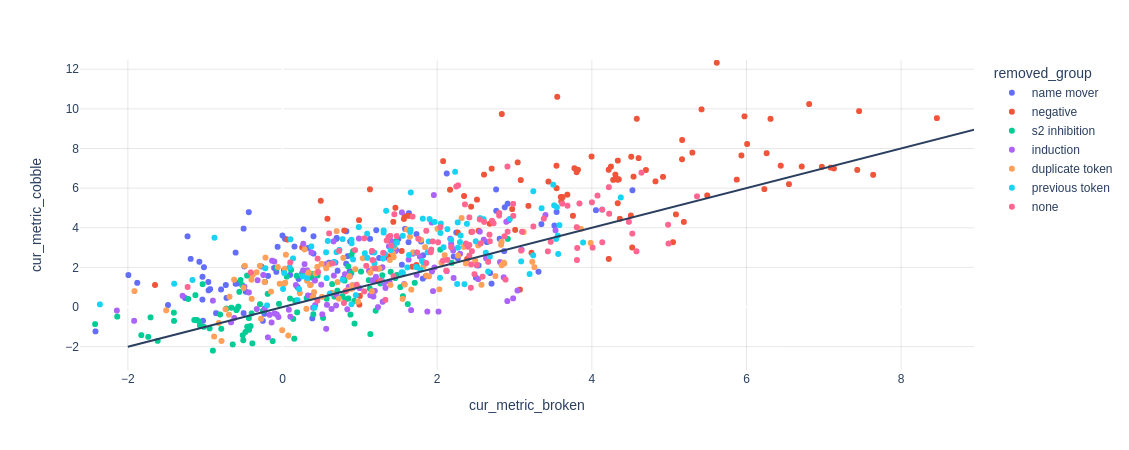
\includegraphics[width=0.65\textwidth]{figs/scatta_zoom.png}
% \end{center}
% \caption{Plot of points $(F(M \setminus K), F(C \setminus K))$, indeed clustered around the line $y=x$ and suggesting completeness. $N=100$ dataset examples, for each circuit classes $G$.}
% \label{fig:completeness}
% \end{wrapfigure}

\begin{figure}
    \centering % cant make these squeeze together : (
     \begin{subfigure}[b]{0.39\textwidth}
         \centering
         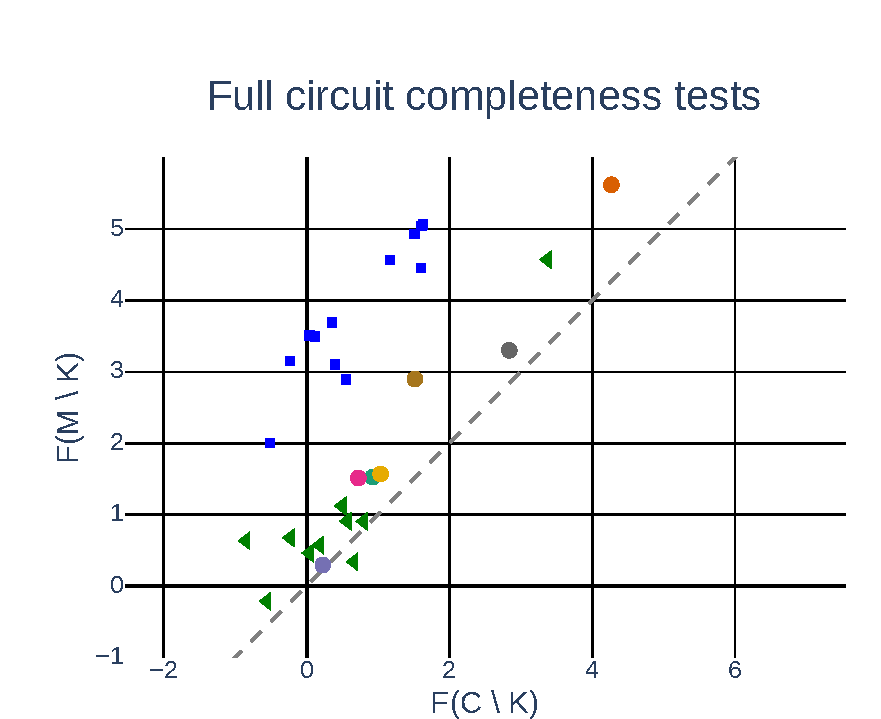
\includegraphics[width=\textwidth]{figs/CompleteLeft.pdf}
         \caption{}
         
         \label{fig:completenessA}
     \end{subfigure}
     \hfill
     \begin{subfigure}[b]{0.51\textwidth}
         \centering
         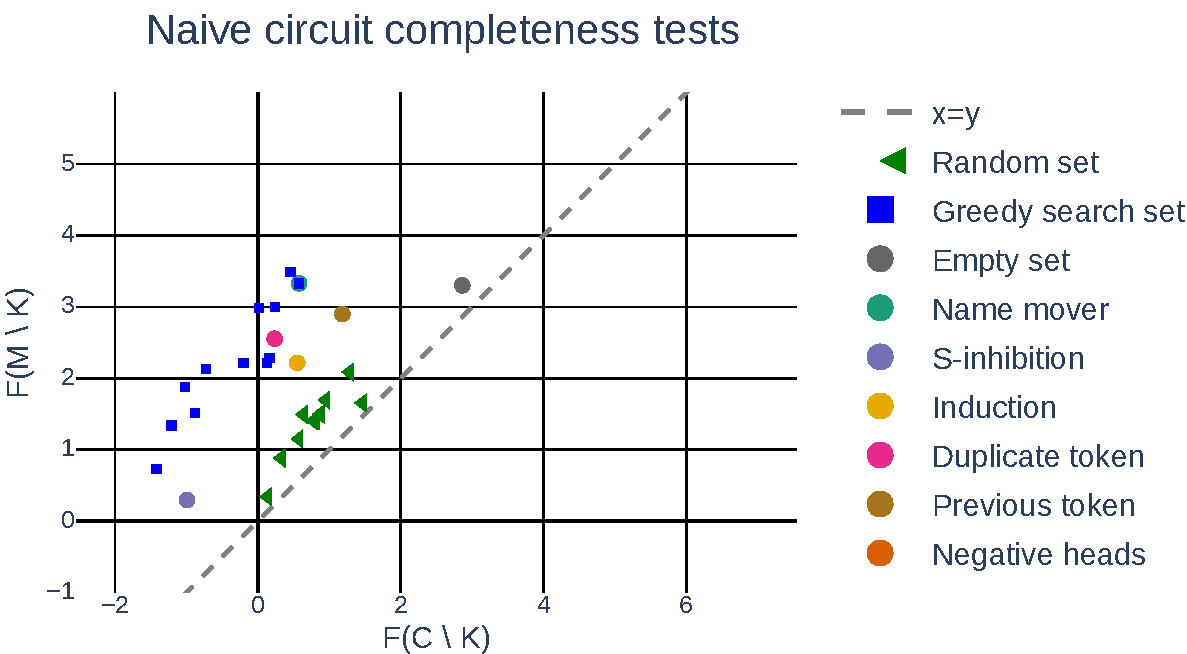
\includegraphics[width=\textwidth]{figs/CompleteRight.pdf}
         \caption{}
         \label{fig:completenessB}
     \end{subfigure}
    \caption{Plot of points $(x_K, y_K) = (F(C \setminus K), F(M \setminus K))$ for (a) our circuit and (b) a naive circuit. Each point is for a different choice of $K$. We show sets $K$ obtained from different sampling strategies: 10 uniformly randomly chosen $K \subseteq C$, $K = \emptyset$, $K$ a class of heads from the circuit, and 10 $K$ found by greedy optimization. Since the incompleteness score is $|x_K - y_K|$, we show the line $y=x$ for reference.}
    \label{fig:completeness}
\end{figure}

\subsection{Minimality}
\label{sec:minimality}

A faithful and complete circuit may contain unnecessary components, and so be overly complex. %For instance, $M$ is a faithful and complete circuit but doesn't give any interpretability insights because it contains nodes irrelevant for the behavior. For a circuit to be a useful explanation, 
To avoid this, we should check that each of its nodes $v$ is actually necessary. %has a counterfactual impact on $F$. 
This can be evaluated by showing that $v$ can significantly recover $F$ after knocking out a set of nodes $K$. 

Formally, the \textbf{minimality} criterion is whether for every node $v\in C$ there exists a subset $K \subseteq C \setminus \{v\}$ that has high \emph{minimality score} $|F(C \setminus (K \cup \{ v \})) - F(C \setminus K)| $. %We call a circuit $A$-\textbf{minimal} if this holds. Alexandre: I fixed some inconcistency because we did not introduced epsilon-complete before, so did not makes sense to introduce A-minimal, right? I think we chose to go for informal argument? A-MINIM (key word to ctrl+F to recover the A-minimality definition).

% \label{eqn:minimality}
% \end{definition}



In the running example, we can show that $C_1 \cup C_2$ is minimal. The proof has two symmetrical cases: $v \in C_1 $ and $v\in C_2$. Without loss of generality, we chose $v \in C_1$, and then define $K = C_2$. The minimality score for this choice of node $v$ and set $K$ is equal to $|F(C_1 \setminus \{ v\}) - F(C_1)|$, which is large since $C_1$ is a serial circuit and so removing $v$ will destroy the behavior.


% Alexandre: I rewrote it to removed the A-minimality A-MINIM.
% ARTHUR REWROTE TO MAKE CLEARER

%In the running example, $C_1 \cup C_2$ is $A$-minimal for some non-trivial $A$. We can sketch a proof of this result given an informal defintion of `non-trivial'. The proof has two symmetrical cases: $v \in C_1 $ and $v\in C_2$. Without loss of generality, $v \in C_1$. We can choose $K = C_2$ and the minimality score is equal to $|F(C_1 \setminus \{ v\}) - F(C_1)|$ which is large since $C_1$ is a serial circuit and so removing $v$ will destroy the behavior.

% OLD SUPER LONG MATH:
% $|F(C \setminus (K \cup \{v_1\} )) - F(C\setminus K)| = |F( C_1\setminus  \{v_1\}) - F(C_1)|$

% However, a complete circuit may still not be `correct' as an explanation, and we would want to make it as small as possible while still being complete. \todo{can extend this?}
% \begin{comment}
% \begin{itemize}
% \item \textbf{Minimality}: a circuit is minimal if 
 
% \begin{equation}
%     \forall v \in C, \exists K \subseteq C, |F( (C \setminus K) \cup \{v\}) - F( (C\setminus K))| \geq A.
% \label{eqn:minimality}
% \end{equation}
% \end{itemize}
% \end{comment}


% Finally, we also wish to understand the actual operations performed by the nodes. We therefore add a qualitative criterion of \textbf{legibility}: every component of $C$ cleanly corresponds to a component of a human-understandable causal model. To check legibility, we provide an explanation of the human-understandable algorithm that $C$ implements and verify this with causal interventions (Section \ref{sec:legibility}). 
% END THE EDIT IN

% \todo{probably we are doing the backup name mover stuff in a fairly different way now...}
% The experiments regarding the Backup Name Movers in Section~\ref{sec:distributed_name_movers} show that it is easy to miss components of a circuit. Have we missed any more components of the circuit, or does our circuit contain unnecessary components? Here, we carefully check that the answer is no, by using the completeness and minimality criteria from Section~\ref{sec:criteria}.

What happens in practice for our circuit? We need to exhibit for every $v$ a set $K$ such that the minimality score is high. %at least $A$ A-MINIM. 
For most heads, removing the class of heads $G$ that $v$ is a part of provides a reasonable minimality score, but in some instances a more careful choice is needed; we provide full details in Appendix \ref{app:minimality} and display final results in Figure~\ref{fig:naive_minimality}. The importance of different nodes varies, but all have a nontrivial impact (at least 1\% of the original logit difference). These results ensure that we did not interpret irrelevant nodes, but do show that the individual contribution of some attention heads is small. %  individual values are not crucial as we interpret the behavior of nodes acting as groups.

%find a subset $K \subseteq C$, for each $v \in C$. We use a heuristic as in the completeness section, though note that since we only need show existence this is sufficient (we don't need perform an intractable search).

% Recall the definition of \textbf{minimality}: $\forall v \in C, \exists K \subseteq C, |F( (C \setminus K) \cup \{v\}) - F( (C\setminus K))| \geq A $. Like in the completeness section, for a given $v \in C$ we first choose $K$ to be the circuit class $G$ that contains $v$. This is because we expect $|F( (C\setminus K)) - F(C)|$ to be large and $|F((C \setminus K) \cup \{v\}) - F(C)|$ to be small, since $C \setminus K$ lacks a crucial component of the causal graph defining circuit behaviour, while adding back $v$ completes the causal graph (with a lower effect size). Indeed, for all heads other than name mover heads, we observe that $F((C \setminus K) \cup \{v\})$ is closer to $F(C)$ than $F(C \setminus K)$, by at least $0.1507$.

\begin{figure}[t]
    \centering
    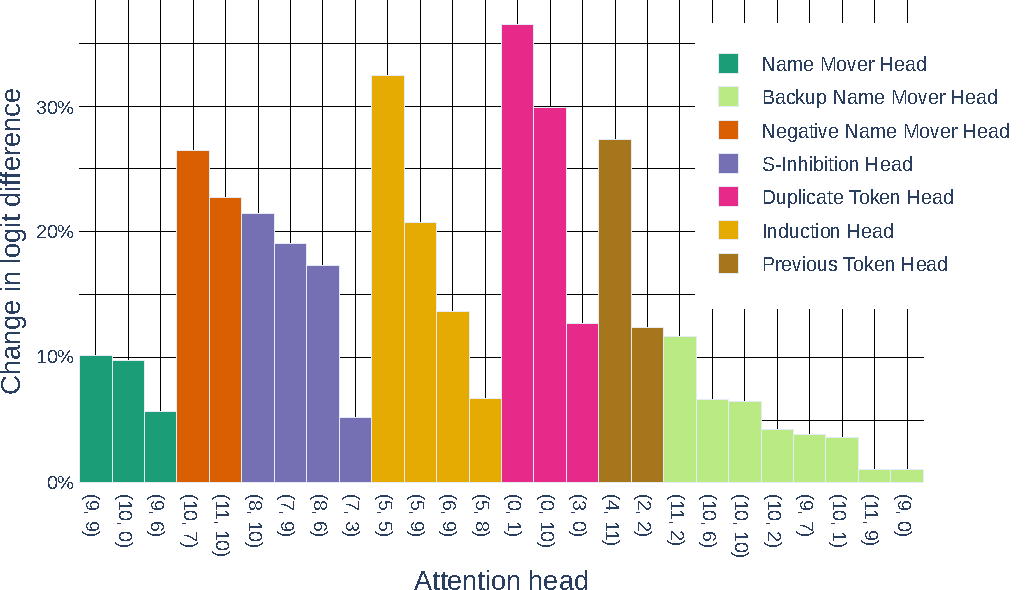
\includegraphics[width=0.9\textwidth]{figs/minimality.pdf}
    \caption{Plot of minimality scores $|F(C \setminus (K \cup \{v\})) - F(C\setminus K)|$ (as percentages of $F(M)$) for all components $v$ in our circuit. The sets $K$ used for each component, as well as the initial and final values of the logit difference for each of these $v$ are in Appendix \ref{app:minimality}. %Our circuit is 0.06-minimal. A-MINIM
    }
    \label{fig:naive_minimality}
\end{figure}

\subsection{Comparison with a baseline circuit}
\label{sec:circuit_extr_validation}

In the previous sections, we evaluated our circuit on three quantitative criteria. 
%But without a relative comparison, these numbers are not particularly useful. 
To establish a baseline for these criteria, we compare to a na\"{i}ve circuit that consists of the Name Mover Heads (but no Backup nor Negative Name Mover Heads), S-Inhibition Heads, two Induction Heads, two Duplicate Token Heads, and the Previous Token Heads. This circuit has a faithfulness score of 0.1, comparable to the full circuit $C$. However, the na\"{i}ve circuit can be more easily proven incomplete: by sampling random sets or by knocking-out by classes, we see that $F(M\setminus K)$ is much higher than $F(C\setminus K)$ (Figure \ref{fig:completenessA}). Nonetheless, when we applied the greedy heuristic to optimize for the incompleteness score, both circuits have similarly large incompleteness scores. %Thus, we conclude that our worst-case completeness criteria was too high a bar for our circuit to meet and future work could use it as a high standard to validate circuit discovery. 


\subsection{Designing adversarial examples}
%\av{Maybe to put in appendix} \ac{I think yes, do this}
%Beyond our criteria, we also tried to validate our findings more directly. 
As argued in \citet{interp_survey}, one way to evaluate the knowledge gained by interpretability work is to use it for downstream applications. In this section, we do this by using knowledge of the circuit to construct simple adversarial examples for the model. 
%For instance, this can be done by designing adversarial examples hard to find without knowing how the model works internally. This is the goal of this section.

%\textbf{Adversarial datasets}
As presented in Section \ref{sec:legibility}, the model relies on duplicate detection to differentiate between S and IO. %The fact that S is duplicated causes Name Mover Heads to attend less to its first occurrence, S1, and ultimately predict IO as more probable than S.
Motivated by this, we constructed passages where both the S and IO tokens are duplicated. An example is ``John and Mary went to the store. Mary had a good day. John gave a bottle of milk to''; see Appendix~\ref{app:advexes_templates} for full details. We find that this significantly reduces the logit difference and causes the model to predict S over IO $23\%$ of the time (Figure~\ref{table:advexes_results}).
%Because Mary is duplicated, this would cause Name Mover Heads to attend less to it, and lead the model to predict a lower probability for ``Mary''. 

To ensure that the observed effect is not an artifact of the additional sentences, we included a control dataset using the same templates, but where the middle sentence contains S instead of IO. In these sentences, S appears three times in total and IO only appears once. On this distribution, the model has an even higher logit difference than on $\pioi$, and predicts S over IO only $0.4\%$ of the time.


%We also designed a more artificial variation of this idea with sentences where the duplicated IO is not part of a meaningful sentence, e.g. ``John and Mary went to the Store. Mary. John gave a bottle of milk to''. The templates used for the adversarial examples are presented in appendix \ref{app:advexes_templates}.

% \textbf{Results of the attack}

% The performance of GPT-2 small on the two adversarial datasets are summarized in the Figure \ref{table:advexes_results} (last two lines). We observe a drop in performance for both datasets, showing that the attack is successful.


\begin{figure}
\begin{center}
\begin{tabular}{ |c|c|c|c|} 
\hline
\textbf{Distribution} & \textbf{Logit difference} & \textbf{IO probability} &  \textbf{\specialcell{ Proportion of\\S logit greater than IO}}\\ 
\hline 
$\pioi$ & 3.55 & 0.49 & 0.7\%  \\
\hline
\specialcell{Additional occurrence of S\\(natural sentence)} & 3.64 & 0.59 & 0.4\% \\
\hline
\specialcell{Additional occurrence of IO\\(natural sentence)} & 1.23 & 0.36 & 23.4\% \\
\hline
%\specialcell{Additional occurrence of IO\\(single-name sentence)} & 0.42 & 0.29 & 43.4\% \\
%\hline
\end{tabular}
\caption{Summary of GPT-2 performance metrics on the IOI task on different datasets. In the line order: for $\pioi$, for the dataset where we added an occurrence of S (thus S appears three times in the sentence) and for the adversarial dataset with duplicated IO in natural sentences.}
\label{table:advexes_results}
\end{center}
\end{figure}


\textbf{Limitations of the attack.}
Despite being inspired by our understanding of our circuit, those examples are simple enough that they could have been found without our circuit with enough effort. 

Moreover, we do not have a full understanding of the mechanisms at play in these adversarial examples. For instance, the S-Inhibition Heads attend not only to S2, but also to the second occurrence of IO. As this pattern is not present in $\pioi$ nor in $\pabc$, it is beyond the analysis presented in Section \ref{sec:legibility}. The study of the behavior of the circuit on these adversarial examples could be a promising area for future work.

% Moreover, our work suggests that greedy sampling is easily able to find limitations of explanations.
% strategies can be useful to quantify progress toward a complete explanation.
% However, as shown in Figure (\ref{fig:completeness}) left, applying the heuristics described above lead to finding sets with completeness score higher than $2.7$. \todo{average estimations?}

%The Figure \ref{fig:completeness} shows that the completeness metric was a high bar to reach \todo{Mention that the new informal definition makes things less brutal}

% % For the name mover heads, all but 9.0, 11.1 and 11.9 meet the $A=0.14$ standard, and as expected cause increases in logit difference. As described in Section \ref{sec:distributed_name_movers}, 11.9 and 11.1 are heads that appear to write both names into the residual stream, and hence the behavior observed is expected. This suggests that instead if $F$ is the IO probabilities metric 

% For a naive circuit, we see far weaker effect sizes:

% \begin{figure}[H]
%     \centering
%     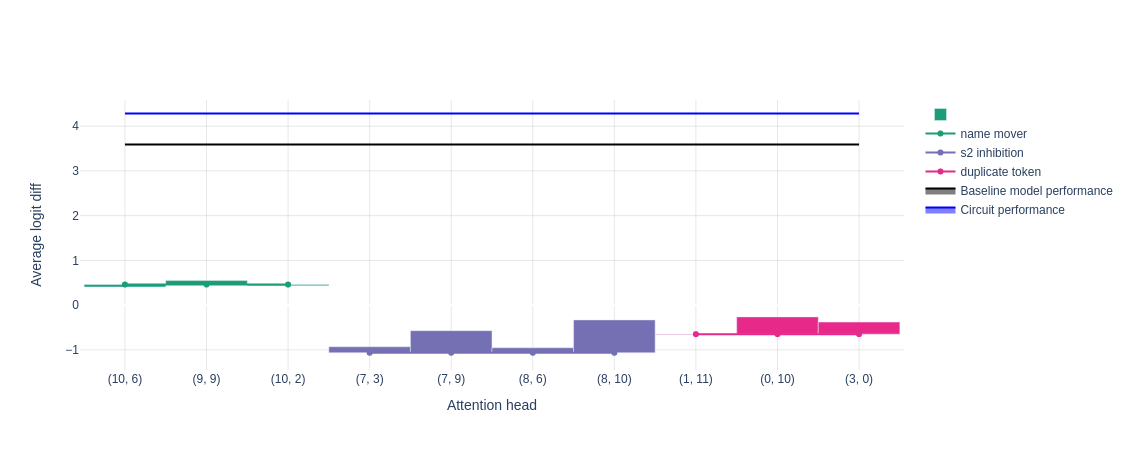
\includegraphics[scale=0.3]{figs/naive_minimality.png}
%     \caption{Same as figure \ref{fig:minimality}, but for the naive circuit.}
%     \label{fig:minimality}
% \end{figure}

% [TODO give analysis of minimality results]

% \subsection{Are Our Tests Strong Enough?}

% We establish a baseline by presenting a naïve circuit $C'$ that passes the faithfulness test: with just NMHs 10.6, 9.9 and 10.2, \todo{rest} we get logit difference (knocking out on the IOI dataset) $F(C') = 4.28$. Since $F(M) = 3.59$ and $F(C) = 4.58$, by the faithful metric, this circuit is better at explaining the model behavior. We argue that completeness and minimality are better tests, in that they are both reasonable standards that an explanation should meet, and they are able to differentiate between circuits that both achieve similar faithfulness scores. \ac{these $F$ values are quite dependent on dataset ... these were generated with the IOI dataset but perhaps we use ABCA in the rest of the work} 


% \todo{use greedy algorithm on minimality}

%OLD CIRCUIT DEFINITION STUFF

% \subsection{Circuit definition}

% \todo{make this flow better with the introduction of the naive circuit just mentioned. Diagram?}
% In full generality, we could consider each node of the computational graph implemented by a transformer as a succession of matrix multiplication and non-linear function. However, we used a more coarse-grained modelisation to express our empirical findings. More precisely, we are interested in understanding the mechanism responsible for information moving across token position. Attention heads are the units responsible for this role, this is why we consider nodes as being pairs $(h, \text{IND})$ where $h$ is an attention head and $\text{IND}$ a token position, as describe in the Section \ref{sec:ablation}. The MLP and LayerNorm are not part of the computational circuit we consider. Those modules are always fully functional in our validation experiments. We also motivate this choice in Appendix \ref{app:mlp} where we present several experiments suggesting a minimal role of the MLP for the IOI task.


% For $F$, we generally use the average logit difference (see Section \ref{sec:metrics}), though verify our explanations are not too dependent on this metric by checking the IO probabilities, too.

% % TODO: ablations last
% % and 2.2 improvements: do things with making more specific to transformers 
% % ablations later 
% % back reference equations
% % not HYPOTHESISE, do the computationally intractable
% % do completeness, minimality NOT methods first
% % 

% \subsection{Circuit extraction}

% The computational graph abstraction as introduced in Section \ref{sec:explanation} cannot be naively transposed to transformers. In particular, for a circuit $C\subseteq M$, computing $F(C)$ by excluding every node from $M\setminus C$ is equivalent to perform zero-ablation on those nodes. This is surely not a great way to represent the absence of features from $M\setminus C$, as a zero activation is likely to be far from the natural computation and introduced corrupted computation in latter nodes. \ac{can't this section just cite \ref{sec:ablation} / that section cite this section? I don't think both are needed}

% To counteract these effects, we used in-template mean ablation to perform \emph{circuit extraction}. We build a circuit $C$ from $M$, by in-template mean ablating every node $(h, \text{IND}) \in M\setminus C$. This as for effect to remove the values of tokens in a particular sentence (e.g. the fact that the indirect object is `John`) while preserving the features linked to the structure of the sentence and the token position (e.g. the fact that the second token is a name). 

% Those restriction can be perceived as too permissive, however as we show in Section \ref{sec:circuit_extr_validation} they preserve a significant amount of specificity. We show that a faithful and legible circuit that doesn't seem to miss any part to fully explain the behavior can fail our minimality and completeness test. This demonstrates that our technique is an effective way to evaluate explanation beyond appearances. This technique also enable to clearly define the scope of the investigation and could enable an incremental study of circuits by dividing the interpretability approach into tractable sub-goals that can be rigorously validated.

% \subsection{Set search}

% The definition of minimality and completeness described in \ref{sec:criteria} rely on an exhaustive search among subset of the circuit. Such an exhaustive search is not computationally tractable. 

% \textbf{Completeness} 
% A first approach is to use the division of heads into classes. Because classes perform similar function, removing them from the model is likely to identify node in $M\setminus C$ that could replace them.


% Alternatively, to ensure that $\forall K \subseteq C, |F(C \setminus K) - F(M \setminus K)| \leq \epsilon$ we can an adversarial approach against the circuit $C$ by greedily optimizing for $K$ node by node to maximize $|F(C \setminus K) - F(M \setminus K)|$. \av{Add the pseudo-code ? not the most intresting but can be included in appendix}
% This method gives us a lower bound on the actual completeness score that depends on the quality of the greedy search. However, we empirically found that the greedy search performed better than the approach by class making us confident that it is able to find good proxy for the global optimum.

% \textbf{Minimality} 
% The minimality criterion only require us to exhibit for every $v$ a certificate set $K$ such that $|F( (C \setminus K) \cup \{v\}) - F( (C\setminus K))| \geq A$. Again, most of the time this certificate can be guessed from the organization by class. If we remove the class of head $G$ and consider $C \setminus G$ with $v \in G$, it is likely that $|F( (C \setminus G) \cup \{v\}) - F( (C\setminus G))|$ will be significant is $v$ is able to partially recover the function of the class $G$ and if $\mathrm(F)(C)$ depend on this ability.
% \label{sec:criteria}

% --------------------------------------
% Blackboxing MLPs, LN, etc.
% --------------------------------------
% scope of what we understand
\begin{comment}
\ac{I think this writing should be moved to the explanation criteria intro if it's wanted - I feel we should be just doing validation in this section}
NLP is notoriously hard to interpret as we would expect a huge number of heuristics such as bigram statistics \todo{cite layer zero transformer}. 
We are blackboxing things that are constant in the distribution (attention patterns) and MLPs.
But we also show that the MLPs aren’t that important
And that attention patterns are distributed
We’re trying to explain the information flow across token positions of information that varies in the distributions, in other words, where the name information flows.
MLPs are notoriously hard to study.
To make the problem tractable, we reduced the scope of the explainable. The scope of our understanding:
\begin{itemize}
    \item We focus on understanding the mechanism that move information across token position. In particular, we did not investigate the MLPs that process information at certain token position.
    \item We tried . This means that we do not investigate the features that are constant in the distribution. 
\end{itemize}
\end{comment}
